
\chapter{GİRİŞ}
Bu bölümde tez konusuyla ilgili olarak hazırlayıcı bilgiler verildikten sonra araştırmanın amacı ve kapsamı açıkça belirtilmelidir. Ayrıca, eğer tez konusu ile ilgili olarak söz edilmek istenen önceki çalışmalar varsa, bunlar da GİRİŞ bölümü içinde verilebilir. Tezin tamamında ana bölümlerin ve alt bölümlerin ilk paragrafının yazımı için "FBE İlk Paragraf" stili seçilmelidir. Seçilen stiller hiçbir şekilde güncellenmemelidir.

Eğer tez çalışmasında ve yazımında olağandışı ve/veya tartışmalı bir adlandırma, sınıflama ve kavram kullanılmışsa, bunların açıklaması yine GİRİŞ bölümünde verilmelidir. Tezin tamamında bölüm ve alt bölümlerin ilk paragraf haricindeki paragrafları için "FBE Paragraf" stili seçilmelidir.

\section{İkinci Dereceden Başlık}
\noindent Tezin herhangi bir sayfasında metnin içinde yazılması halinde konuyu dağıtıcı ve okumada sürekliliği engelleyici nitelikteki çok kısa ve öz açıklamalar birkaç satır halinde aynı sayfanın altına dipnot olarak verilebilir. Dipnotlar sayfa içindeki ana metinden iki aralık bırakıldıktan sonra, soldan sağa bir çizgi ile ayrılmalıdır. Sayfanın alt kenarında bırakılması gereken boşluğa kesinlikle taşmamalıdır.

Yazılan ilk dipnotta\footnote{Dipnotlar bu örnekteki gibi yazılmalı. İlk dipnot metni için FBE Dipnot Metni İlk Satır stili seçilmelidir.}   şablonda yer alan stiller içerisindeki "FBE Dipnot Metni İlk Satır" stili seçilmelidir. İkinci\footnote{İkinci dipnot. İkinci ve sonraki dipnot metinleri için ise FBE Dipnotlar stili seçilmelidir.}, üçüncü\footnote{İkinci ve sonraki dipnot metinleri için ise FBE Dipnotlar stili seçilmelidir.} ve sonraki dipnotlarda ise satır aralıkları tek satır olarak ayarlanmalıdır. İkinci ve sonraki dipnotlar için "FBE Dipnotlar" stili seçilmelidir.

Dipnot çizgisi ile dipnot numarası arasında bir aralık boşluk bırakılmalıdır. Dipnot simgesi Arabic rakam olarak seçilmeli ve dipnot simgesinden sonra bir boşluk bulunmalıdır. Dipnotun açıklaması bir satır aralığı ile yazılmalı ve 8 punto kullanılmalıdır. Dipnotlar her sayfa içinde belirme sırasına göre "1" den başlayarak numaralandırılmalı ve dipnot açıklaması mutlaka değinilen sayfada yer almalıdır. 

\subsection{Sayıların Yazılışı}
\noindent Bir zorunluluk olmadıkça cümle rakamla başlamamalıdır.

Dört veya daha çok basamaklı sayılar sondan sayılmak üzere üçlü gruplara ayrılarak yazılmalı ve aralarına nokta konulmalıdır:

Örnek: 3.822 (Üç bin sekiz yüz yirmi iki)

196.995 (Yüz doksan altı bin dokuz yüz doksan beş)

81.250.124 (Seksen bir milyon iki yüz elli bin yüz yirmi dört )

Dört veya daha çok basamaklı sayıların kolay okunabilmesi amacıyla içinde geçen bin, milyon, milyar ve trilyon sözleri harfle yazılabilir.

Örnek: 12 trilyon 300 milyar 245 milyon 595 bin (12.300.245.595.000)


\subsubsection{Kesirlerin yazılışı}
\noindent Sayılarda kesirler virgülle ayrılmalıdır.

Örnek: 12,7 (12 tam, onda 7)

Bayağı kesirlere getirilecek ekler alttaki sayı esas alınarak yazılmalıdır.

Örnek: 2/3’ü (iki bölü üçü), 1/7’si (bir bölü yedisi).

Birbirini takip eden ondalık sayılar noktalı virgül ";" ile ayrılmalıdır.

Örnek: 12,7; 9,45; 2,11 vb.

Yüzde ve binde işaretleri yazılırken sayılarla işaret arasında boşluk bırakılmamalıdır.

Örnek: \%25, \textperthousand 50 vb.


\subsection{Çizelge Örneği}
\noindent Tezin yazımında kullanılabilecek iki tip çizelge aşağıda verilmiştir. Çizelge başlıkları için "FBE Çizelge Yazısı" stilini kullanınız. Çizelge ve numarası kalın yazılmalıdır. Tablo içindeki metin için "FBE Tablo İçi Yazı" stilini kullanınız. Çizelge içinde verilen açıklamalar için kullanılacak stil ise "FBE Tablo Dipnotları"dır.

\begin{table}[!t]
	\caption{Çizelge başlığı cümle sonuna nokta konulmadan iki yana yaslı olarak bölüm numarası ile birlikte yazılmalıdır}
%\begin{adjustbox}{width=1\textwidth}
	\begin{tabular}{L{3cm}L{3cm}L{3cm}L{3cm}}
		\hline\hline
		Başlık&Başlık&Başlık&Başlık\\\hline
	A&&&\\
	B&&&\\
	C&&&\\
	\hline\hline
	\end{tabular}
%\end{adjustbox}
\vspace{24pt}
\end{table}


\begin{table}[!t]
	\caption{Örnek tablo 2}
	\begin{tabular}{L{3cm}L{3cm}L{3cm}L{3cm}}
	\hline
	Başlık&Başlık&Başlık&Başlık\\\hline
	A&&&\\
	B&&&\\
	C&&&\\
	\hline
\end{tabular}
\vspace{24pt}	
\end{table}

	
Çizelgelerden sonra yazılacak ilk paragraf için kullanılacak stil "FBE Çizelge Sonrası" olmalıdır. Çizelgelerden sonra yazılacak paragrafın çizelge ile arasında 24 nk boşluk olmalıdır. 

\subsection{Şekil Örneği}
\noindent Şekillerin başlık yazısı için "FBE Şekil Yazısı" seçilmelidir ve şeklin altında bölüm numarası ile beraber verilmelidir.

\begin{figure}[!h]
	%\centering
	
\includegraphics[width=0.2\linewidth]{sekiller/nku_logo}
	\caption{Şekil başlığı cümle sonuna nokta konulmadan iki yana yaslı olarak bölüm numarası ile birlikte yazılmalıdır}
	\label{fig:nkulogo}
	\vspace{24pt}
\end{figure}

Şekillerden sonra yazılan paragraflar ile şekil yazıları arasındaki boşluk 24 nk olmalıdır. 

\begin{figure}
	%\centering
	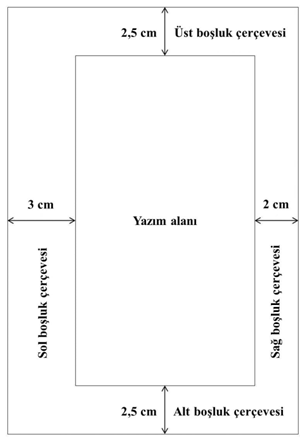
\includegraphics[width=0.2\linewidth]{sekiller/sekil}
	\caption{Örnek şekil yazısı 2}
	\label{fig:sekil}
	\vspace{24pt}
\end{figure}

\subsection{Denklem Örnekleri}
\noindent Denklem yazarken denklemler sayfayı ortalamış, numarası da sayfanın sağına yaslanmış olmalıdır. Bunu sağlayabilmek için kenarlığı olmayan bir tablo kullanılabilir.
\begin{equation}
f(x)=a_0+\sum_{n=1}^{\infty}\left(a_n\cos\frac{n\pi x}{L}+b_n\sin\frac{n\pi x}{L}\right)
\end{equation}
\begin{equation}
a^2+b^2=c^2
\end{equation}

Denklemlerden sonra paragraf buradan başlar, "FBE Paragraf" stili kullanılmalıdır.






\subsection{Madde İşaretleri ve Numaralandırma}
\noindent Madde işaretleri 1,25 cm içeriden ve 1,75 sekme durak yeri ile yapılmalıdır. Bunun için kısa yol stili olarak "FBE Madde İşaretleri" sekmesi seçilebilir.
\begin{itemize}
	\setlength{\itemindent}{1.25cm}
	\item Örnek işaretlenmiş metin 1
    \item Örnek işaretlenmiş metin 2
     \item Örnek işaretlenmiş metin 3
     \item Örnek işaretlenmiş metin 4
\end{itemize}

Madde numaralandırma 1,25 cm içeriden ve 1,75 sekme durak yeri ile yapılmalıdır. Bunun için kısa yol stili olarak "FBE Numaralandırma" sekmesi seçilebilir.
\begin{enumerate}
	\setlength{\itemindent}{1.25cm}
	\item Örnek numaralandırılmış metin 1
	\item Örnek numaralandırılmış metin 2
	\item Örnek numaralandırılmış metin 3
	\item Örnek numaralandırılmış metin 4
\end{enumerate}

Metnin herhangi bir yerinde geçen Latince kelimeler için "FBE Latince" stili kullanılmalıdır.


\section{Kaynak gösterme}

\subsection{"Soyadı Yıl" Kaynak Gösterme Tekniği}

Bu teknikte kaynak gösterme “Yazarın Soyadı Yayın Yılı” sistemine göre yapılmalıdır. Soyadından sonra virgül “,” koymadan bir karakter boşluk bırakılmalıdır.

Tek yazarlı bir eser metin içinde kaynak gösterildiğinde \parencite{Olekseyuk2002} şeklinde, iki yazarlı bir eser kaynak gösterildiğinde \parencite{Yoo2010} şeklinde, üç ve daha fazla yazarlı bir eser kaynak gösterildiğinde \parencite{Sakamoto2005} şeklinde cümlenin sonuna bir atıf yapılmalıdır.

Kaynak, cümle içerisinde kullanılıyorsa kaynağın sadece yılı parantez içerisinde gösterilmelidir.

Örnek: \citet{Sakamoto2005} yıllık yağış miktarının düşük olmasının ........dan kaynaklandığını ifade etmişlerdir.
Bir diğer kaynak gösterme/değinme biçiminde, yazarın soyadına göre “a” ve “e” takıları eklenmelidir.

Örnek: \citet{Olekseyuk2002}’a göre verim parametrelerinde meydana gelen azalmanın sebebi kuraklıktır.
Aynı anda birden fazla eser kaynak gösteriliyorsa, bunlar kronolojik olarak sıralanmalı ve yayın araları “,” (virgül) ile ayrılmalıdır. Aynı yıla ait farklı yazarların kaynakları harf sırasına göre sıralanmalıdır. Aynı yazarın değişik tarihlerdeki yayınlarına aynı anda değinme yapılıyorsa, yayınlar tarih sırasına göre eskiden yeniye doğru “,” (virgül) ile ayrılarak sıralanmalıdır. Aynı yazarın aynı tarihteki yayınlarına tez içerisinde muhtelif yerlerde değiniliyorsa, kullanım sırasına göre birinciden başlayarak yayın yılının sonuna “a, b, …” gibi küçük harfler konulmalıdır. Örnek: ........... olduğu yapılan çalışmalardan anlaşılmıştır (Şirin ve ark. 2003, 2009, Kaya 2006, Aras 2007a, 2007b, Arı ve Güneş 2007, Özdil 2015).
Kaynak bir başka eser içinde kaynak şeklinde bulunuyorsa ve bilginin yer aldığı ilk yayın elde edilememişse, bu aşağıdaki şekillerden biriyle yazılmalıdır:

1. Demir ve ark. (2002) tarafından bildirildiğine göre ……..… bu yöntem ilk defa Aksöz (1954) tarafından kullanılmıştır.

2. ........... uygulanan yöntem Yalçın (1980) tarafından kullanılmıştır (Yılmaz 2006).

3. Aksöz (1954) tarafından kullanılan yöntem .......... keşfedilmiştir (Demir ve ark. 2002).
Bir komisyon ya da kurum tarafından hazırlanan ve yazarı belirtilmeyen yayınlarla kurum ve kuruluşlar tarafından yazarsız yayınlanan kaynaklar “Anonim Yıl” olarak belirtilmelidir. Örnek: Türkiye’de kanatlı eti üretimi artış göstermiştir (Anonim 2007a).

Örnek: ........... istatistiklerine göre (Anonim 2007b) Türkiye’de kişi başına düşen kanatlı eti tüketimi artmıştır.
Tez içinde başka bir kaynaktan alınmış bir bölüm aynen aktarılmak isteniyorsa, bu alıntı ayıraç “...” içinde yazılmalıdır.
Bir başka eserden aynen alınan şekil veya çizelge kullanılacaksa, şekil veya çizelgenin açıklama yazısında “Soyadı Yıl” sistemine göre, gerekliyse yasal izinleri alarak atıf yapılmalıdır. Örnek: Şekil 1.2. ……..… pH üzerine etkisi (Gün ve Ulu 2007)
Örnek: Çizelge 3.5 ............ meydana gelen değişiklikler (Günaydın 2006)

Sözlü ve yazılı görüşmeler metin içerisinde “Soyadı Yıl” sistemiyle belirtilmelidir. KAYNAKLAR dizininde ise kişi ad(lar)ı ve tarih diğer kaynaklar gibi yazılmalı, tarihten sonra sırasıyla yazılı/sözlü görüşme ibaresi ve adres yer almalıdır.





